\documentclass[12pt,a4paper]{article}
\usepackage[T1,T2A]{fontenc}
\usepackage[utf8]{inputenc}
\usepackage[russian]{babel}
\usepackage{indentfirst}
\usepackage[a4paper,top=2cm,bottom=2cm,left=3cm,right=2cm,marginparwidth=1.75cm]{geometry}
\usepackage{graphicx}
\usepackage{titlesec}
\titlelabel{\thetitle.\,\,}
\usepackage{amsmath,amsfonts,amssymb}
\usepackage{float}

\begin{document}
\title{\textbf{Лабораторная работа №6}}
\author{}
\date{}
\maketitle

Пример, в котором направление поиска метода Хука-Дживса шло не лесинкой.
\begin{gather*}
    Q(x) = (x_1^2+x_2^2-11)^2 + (x_1+x_2^2-7)^2+x_1-x_2,\\
    -5 \le x_1 \le 4.5, \; -4.5 \le x_2 \le 5,\\
    x^0=(-0.09, \; 2.9).
\end{gather*}

\begin{figure}[H]
    \centering
    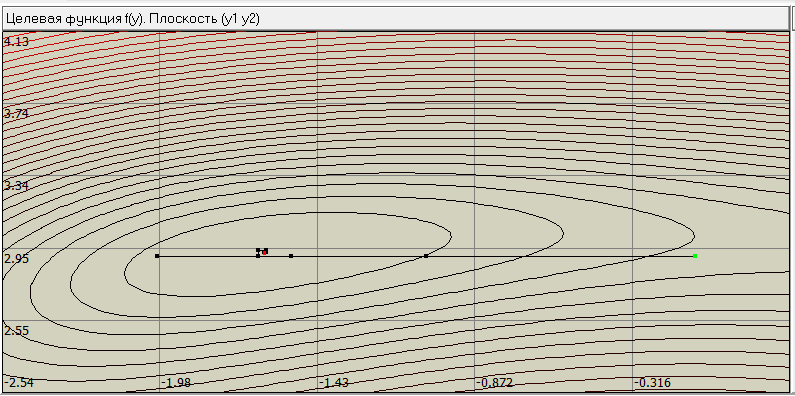
\includegraphics{hj.png}
\end{figure}

Метод Нелдера-Мида на этом же примере.

\begin{figure}[H]
    \centering
    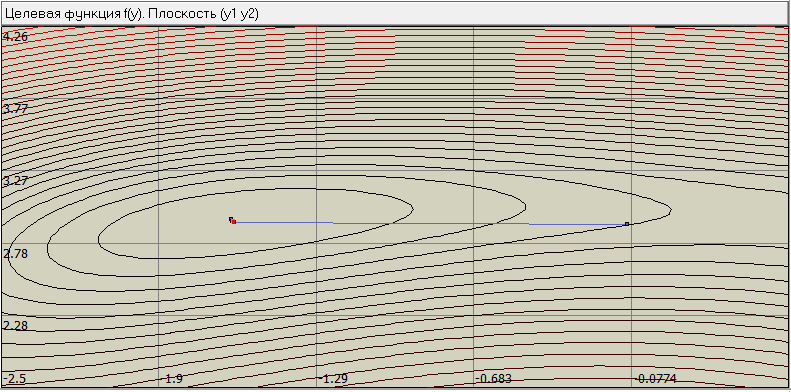
\includegraphics{nm.png}
\end{figure}

Примеры, в которых метод Ньютона, модифицированный метод Ньютона и квазиньютоновский метод ведут себя по разному из одной начальной точки. Метод Ньютона показан синими траекториями, модифицированный -- зелёным, квазиньютоновский -- красным.

\textit{Пример 1.}
\begin{gather*}
    Q(x) = 20(\cos{3x_1}-x_2)^2 + (x_2-4x_1)^2,\\
    -1.5 \le x_1 \le 2, \; -1.5 \le x_2 \le 2,\\
    x^0 = (-1, \; 1.5).
\end{gather*}

\begin{figure}[H]
    \centering
    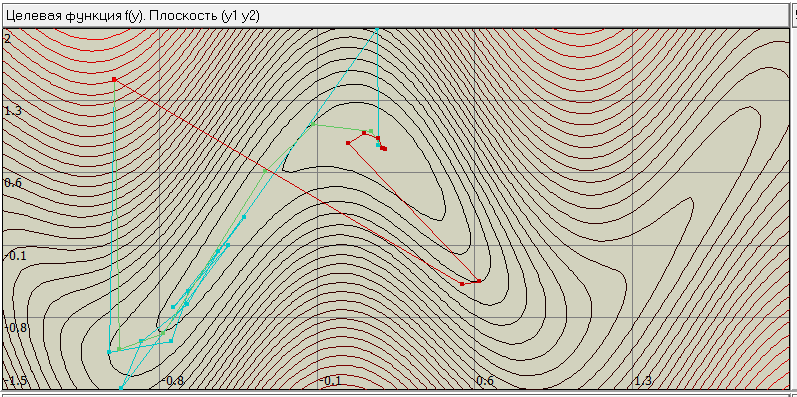
\includegraphics{newton1.png}
\end{figure}

\textit{Пример 2.} Здесь метод Ньютона сошёлся в точку максимума, остальные -- в точку минимума.
\begin{gather*}
    Q(x) = \sqrt{\sqrt{100(x_1-x_2^2)^2 + (x_2-1)^2 + 0.03^2}},\\
    -1 \le x_1 \le 1.5, \; -1.25 \le x_2 \le 1.25,\\
    x^0 = (0.52, \; -0.02).
\end{gather*}        
\begin{figure}[H]
    \centering
    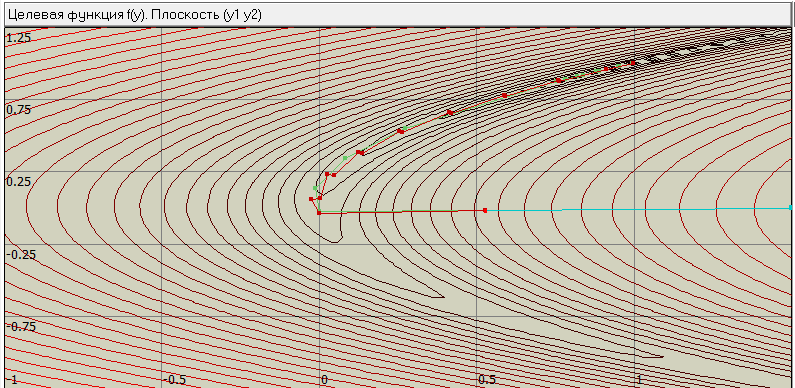
\includegraphics{newton2.png}
\end{figure}

\textit{Пример 3.}
\begin{gather*}
    Q(x) = (x_1^2+x_2^2-11)^2 + (x_1+x_2^2-7)^2+x_1-x_2,\\
    -5 \le x_1 \le 4.5, \; -4.5 \le x_2 \le 5,\\
    x^0=(-1.5, \; 1.5).
\end{gather*}

\begin{figure}[H]
    \centering
    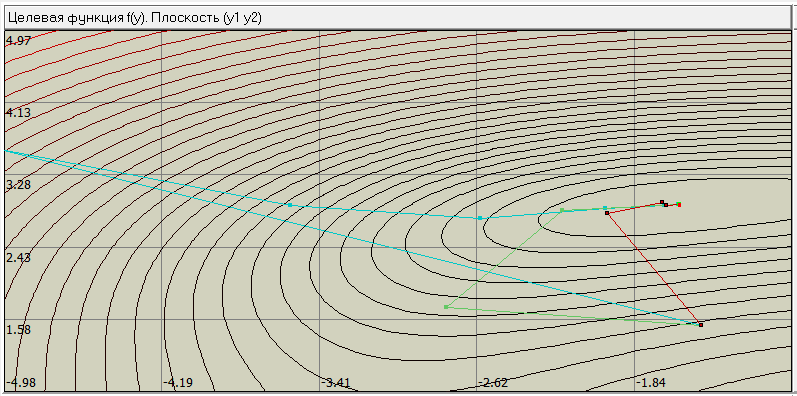
\includegraphics{newton3.png}
\end{figure}

\end{document}